% The Mills page three ways, side by side: the 1947 scan, Mills 8A in
% LuaLaTeX, Mills 8A through standard pdfLaTeX fonts.  render.sh builds this
% (pdflatex, in out/) and joins it with the full-size pages (compare-scan.tex,
% mills-8a.pdf, mills-8a-pdf.pdf) into out/mills-compare.pdf.
\documentclass{article}
\usepackage[paperwidth=93pc,paperheight=52pc,margin=1pc]{geometry}
\usepackage{graphicx}
\pagestyle{empty}
\setlength\parindent{0pt}
\newcommand\panellabel[1]{\par\vspace{6pt}{\small\sffamily #1}\par}
\begin{document}
\centering
\begin{minipage}[t][49pc][t]{29pc}\vspace{0pt}\centering
  \vspace*{1.6pc}% the scan crop has no top margin: align the titles
  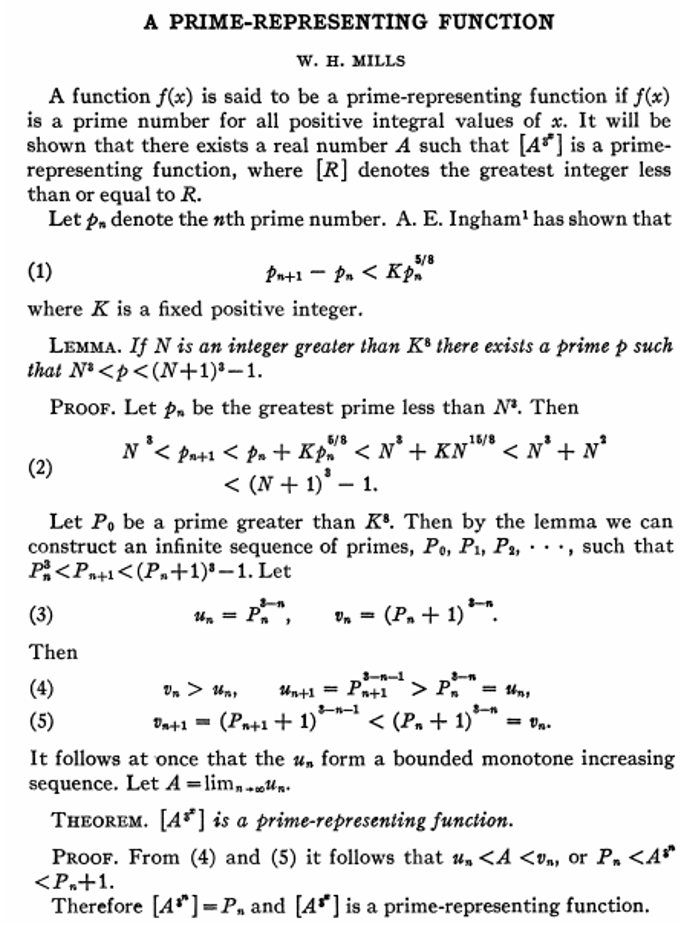
\includegraphics[width=24.6pc]{../scan-mills1947.png}
  \vfill\panellabel{1947 \textit{Bulletin of the AMS} (scan)}
\end{minipage}\hfill
\begin{minipage}[t][49pc][t]{29pc}\vspace{0pt}\centering
  \includegraphics[height=46.5pc]{mills-8a.pdf}
  \vfill\panellabel{Mills 8A, LuaLaTeX (random impressions, wobble)}
\end{minipage}\hfill
\begin{minipage}[t][49pc][t]{29pc}\vspace{0pt}\centering
  \includegraphics[height=46.5pc]{mills-8a-pdf.pdf}
  \vfill\panellabel{Mills 8A, pdfLaTeX (standard Type 1 / TFM fonts)}
\end{minipage}
\end{document}
